\documentclass[conference]{IEEEtran}
\usepackage{amsmath,amssymb}
\usepackage{booktabs}
\usepackage{cite}
\usepackage{graphicx}
\usepackage{url}
\usepackage{xcolor}
\usepackage{balance}

\title{Mission Preservation After Catastrophic Multirotor Damage:\\
A Literature Review and Reproducible Terminal-Descent Framework}

\author{\IEEEauthorblockN{Research Baseline}
\IEEEauthorblockA{Mission-Preservation UAV Project\\
FR-project repository}}

\begin{document}
\maketitle

\begin{abstract}
Catastrophic rotor or actuator damage can remove the possibility of sustained
hover and conventional navigation without removing all useful capabilities.
During the remaining descent, a multirotor may still be able to reduce
horizontal speed, select among reachable terminal regions, point a camera,
transmit data, and preserve the airframe or payload. Existing literature is
strong in individual layers---fault-tolerant control, residual controllability,
landing-site perception, and emergency trajectory planning---but those layers
are rarely optimized as one mission-aware terminal decision problem. This paper
reviews those approaches and proposes a safety-constrained framework that
maximizes residual mission utility only after hard constraints on human
exposure, reachability, and impact state have been enforced. A reproducible
Python baseline is evaluated in three degraded multirotor scenarios. In the
one-rotor-loss experiment, the model reaches ground contact after 20.9 s at a
speed of 1.5 m/s, with the landing-site selector rejecting a high-exposure
urban roof and selecting a reachable communications corridor. The results are
illustrative simulator outputs, not flight-test evidence; they establish a
measurement and experiment structure for future high-fidelity and
hardware-in-the-loop work.
\end{abstract}

\begin{IEEEkeywords}
UAV, multirotor, rotor failure, fault-tolerant control, emergency landing,
terminal control, landing-site selection, mission utility, survivability
\end{IEEEkeywords}

\section{Introduction}
Small unmanned aerial vehicles are increasingly used for inspection, mapping,
communications, and time-critical observation. A rotor fracture, motor
shutdown, power-distribution fault, or actuator saturation can abruptly move
the vehicle outside the envelope assumed by its nominal controller. Treating
this event only as a binary ``continue flight'' or ``land immediately'' problem
loses potentially valuable capabilities. The vehicle may have seconds or
minutes in which it can change its impact location, reduce kinetic energy,
transmit a critical data fragment, orient a sensor, or make its payload more
recoverable.

The central question considered here is:
\emph{given a known or uncertain loss of actuator authority, how should the
vehicle allocate its remaining control, energy, sensing, and communication
resources before terminal contact?} The answer must be safety-first. Mission
value cannot justify intentionally selecting a site with unacceptable exposure
to people or critical infrastructure. Thus, the problem is formulated as a
constrained decision problem rather than as an unconstrained weighted reward.

This paper makes four contributions:
\begin{enumerate}
\item a structured review connecting rotor-loss control, safe landing-site
assessment, wind-aware landing, and emergency decision-making;
\item a formal separation between fault estimation, site feasibility, terminal
mode selection, and degraded control execution;
\item a standard-library Python simulator that makes the assumptions and
metrics reproducible; and
\item quantitative figures and baseline results generated directly from the
repository's JSON experiment outputs.
\end{enumerate}

\section{Background and Related Work}
\subsection{Residual controllability after rotor loss}
Mueller and D'Andrea showed that a quadrocopter can retain useful control after
the complete loss of one, two opposing, or three propellers
\cite{mueller2014loss}. Their strategy accepts continuous rotation around a
body-fixed axis and uses the remaining thrust to move that axis in inertial
space. The important implication is that loss of a rotor does not define a
single outcome: the attainable motion set depends on the failed rotor, thrust
reserve, vehicle geometry, and the control objectives. Their one- and
two-propeller-loss cases were validated experimentally, while the
three-propeller case was evaluated in nonlinear simulation.

Subsequent fault-tolerant-control research has addressed control allocation,
fault estimation, sliding-mode robustness, adaptive compensation, and
controller switching. Uniform fault-tolerant control seeks to avoid abrupt
changes between separately designed controllers after a rotor failure
\cite{shi2022uniform}. Observer-based methods estimate the equivalent
disturbance and redistribute the remaining actuator commands
\cite{dob2026}. A recent systematic review reports that actuator faults and
quadrotor platforms dominate the UAV fault-tolerant-control literature, with
model-based and learning-augmented strategies forming the major families
\cite{ftcReview2026}.

These approaches primarily optimize stability, tracking error, or continued
flight. They provide the execution layer needed by the present framework but
do not normally answer whether residual authority should instead be spent
pointing a payload, transmitting data, or reaching a lower-risk terminal site.

\subsection{Landing-site perception and semantic risk}
Autonomous landing-site assessment commonly combines semantic classification
with geometric measurements. A candidate may be evaluated using slope,
flatness, roughness, obstacle clearance, and surface texture. The visual
environment assessment pipeline in \cite{visualLanding2024} combines
semantic data from a neural network with disparity-derived geometry and
explicitly considers slope, flatness, and roughness. This is preferable to
using image texture alone because a visually uniform surface may still be
sloped, unstable, or obstructed.

Geometry is not sufficient for emergency landing. A flat road, roof, or
parking area may have people, vehicles, power equipment, or other hazards.
Recent context-aware work combines remote-sensing segmentation with
point-of-interest information and vision-language reasoning to identify
semantic hazards not visible in local geometry alone
\cite{hua2026elss}. The resulting design principle is adopted here: geometry
and semantic exposure are separate features, and human exposure is a hard
constraint rather than merely another reward term.

\subsection{Emergency trajectory planning}
Landing-site selection and approach planning are coupled. A safe site that is
outside the reachable set is not a valid option. Recent drone-landing
trajectory work incorporates wind sensing and multiple operational and safety
objectives into reinforcement-learning-based planning
\cite{wang2025wind}. Other risk-aware approaches translate semantic
segmentation into a risk map and integrate it into the landing control loop
\cite{zhang2026risk}. These studies motivate a time-varying reachability test
that includes current velocity, remaining time, degraded acceleration, and
wind.

\subsection{Gap addressed by this project}
The reviewed work can be grouped into four layers:
\begin{enumerate}
\item \textbf{control authority:} what motion remains possible after failure;
\item \textbf{perception:} which surfaces and contexts appear suitable;
\item \textbf{trajectory generation:} how to approach a selected terminal
region; and
\item \textbf{decision utility:} what mission value remains worth pursuing.
\end{enumerate}
The first three layers are increasingly mature, but the fourth is usually
implicit. A mission-preservation policy makes it explicit while retaining
safety gates. It can therefore compare a recoverable landing, a short
transmission opportunity, and a human-exposure-minimizing descent using a
common state and evaluation protocol.

\section{Problem Formulation}
Let the terminal state be
\begin{equation}
x_t=[p_t,v_t,q_t,\omega_t,h_t,e_t,d_t,c_t],
\end{equation}
where $p,v,q,\omega$ are position, velocity, attitude, and angular rate;
$h$ is rotor health; $e$ is remaining energy; $d$ is the data backlog; and
$c$ is communication quality. The action $u_t$ contains a target velocity,
attitude preference, camera orientation request, transmission request, and
the selected terminal region.

The mission objective is
\begin{equation}
\max_{\pi}\ \mathbb{E}_{\pi}\left[
U_{\mathrm{mission}}+U_{\mathrm{data}}+U_{\mathrm{observe}}
 +U_{\mathrm{recover}}-\lambda_E E_{\mathrm{impact}}\right],
\label{eq:objective}
\end{equation}
subject to
\begin{align}
P(\mathrm{human\ exposure})&\leq \epsilon_H,\\
s&\in\mathcal{R}(x_t,h_t,\Delta t),\\
\|\omega_{\mathrm{contact}}\|&\leq \omega_{\max},\\
\|v_{\mathrm{contact}}\|&\leq v_{\max},\\
u_t&\in\mathcal{U}(h_t).
\end{align}
Here $\mathcal{R}$ is the degraded reachable set and $\mathcal{U}$ is the
remaining actuator set. The human-exposure inequality is intentionally
separate from the utility objective. If no site satisfies it, the fallback
mode minimizes exposure and impact energy over the remaining reachable
states.

\section{Proposed Framework}
\subsection{Architecture}
The proposed architecture has five stages:
\begin{enumerate}
\item \textbf{Fault diagnosis:} estimate rotor health and uncertainty from
motor commands, inertial residuals, and thrust response.
\item \textbf{Attainable-control estimation:} compute conservative bounds on
acceleration, angular rate, and descent authority.
\item \textbf{Candidate-site assessment:} score geometry, semantic exposure,
reachability, mission value, communications, and recovery access.
\item \textbf{Terminal-mode selection:} choose human-exposure minimization,
recoverable landing, or bounded transmit-and-observe.
\item \textbf{Execution and fallback:} track the selected velocity/attitude
command and interrupt all secondary tasks when safety margins deteriorate.
\end{enumerate}

\subsection{Reduced-order dynamics}
The current simulator represents health as four thrust fractions
$h_i\in[0,1]$. The effective authority used by the baseline is
\begin{equation}
\alpha=\max\left(0.05,\bar{h}(1-0.35\Delta h)\right),
\end{equation}
where $\bar{h}$ is the mean health and $\Delta h$ is the maximum health
spread. A target velocity is converted to a desired acceleration and bounded
by $a_{\max}=4\alpha$ m/s$^2$. A wind vector is added as a disturbance.
Position is then integrated using a fixed step of 0.1 s. The model maps
velocity to bounded roll and pitch preferences but does not claim to model
full rigid-body aerodynamic coupling.

\subsection{Landing-site score}
Each candidate site has distance, flatness, obstacle clearance, human
exposure, recovery access, mission value, and communication quality. A site is
feasible only if it is reachable, has flatness at least 0.35, clearance at
least 0.4, and human exposure no greater than 0.35. Feasible sites are ranked
by
\begin{equation}
J_s=w_L S_s+w_M M_s+w_R R_s+w_C C_s+w_E G_s,
\end{equation}
where $S_s$ combines flatness, clearance, and inverse exposure, $M_s$ is
mission value, $R_s$ recovery access, $C_s$ communication quality, and $G_s$
is a distance/reachability term. The baseline uses
$[w_L,w_M,w_R,w_C,w_E]=[0.45,0.20,0.15,0.10,0.10]$.

\subsection{Terminal-mode policy}
The baseline selects \texttt{minimize\_human\_exposure} if no feasible site
exists. If a safe site exists and more than 20 percent of the data backlog
remains, communication quality exceeds 0.4, and at least 5 s remain, it
selects \texttt{transmit\_and\_observe}; otherwise it selects
\texttt{recoverable\_landing}. Transmission and observation are thus
opportunistic subtasks with a safety-preserving fallback, not independent
commands that can override the landing constraint.

\section{Experimental Method}
\subsection{Implementation and reproducibility}
The implementation uses Python's standard library for the simulator and
Matplotlib/NumPy only for figure generation. The source is in
\texttt{src/terminal\_uav}; tests are in \texttt{tests}; and the figure
generator is \texttt{scripts/generate\_figures.py}. Every scenario is run
with the same 0.1-s integration step and 30-s maximum horizon. The initial
altitude is 30 m and initial horizontal speed is 3 m/s. The one-rotor-loss
case uses health $(0,1,1,1)$, the two-rotor-loss case uses $(0,1,0,1)$, and
the windy partial-failure case uses $(0.2,0.8,1.0,0.7)$ with wind
$(0.2,-0.1,0)$ m/s$^2$.

\subsection{Metrics}
The current results report:
\begin{itemize}
\item contact time and whether altitude reached zero;
\item contact-speed magnitude as an impact-energy proxy;
\item horizontal terminal displacement;
\item selected site and terminal mode; and
\item sampled altitude, position, and velocity histories.
\end{itemize}
These metrics are not a substitute for human-injury risk, structural impact
testing, or validated aerodynamic prediction. They are baseline observables
for comparing policies before higher-fidelity work.

\section{Results}
\subsection{One-rotor-loss trajectory}
Fig.~\ref{fig:trajectory} shows the generated horizontal trajectory and
altitude history. The one-rotor-loss run begins at 30 m altitude with 3 m/s
horizontal speed. The degraded controller first damps the horizontal motion
and then maintains a commanded descent velocity of approximately
$-1.5$ m/s. Contact occurs at 20.9 s, at approximately
$(2.431,0,0)$ m, with speed 1.5 m/s. The nonzero horizontal displacement
illustrates why site feasibility must consider the trajectory rather than
only the nearest visually suitable point.

\begin{figure*}[t]
\centering
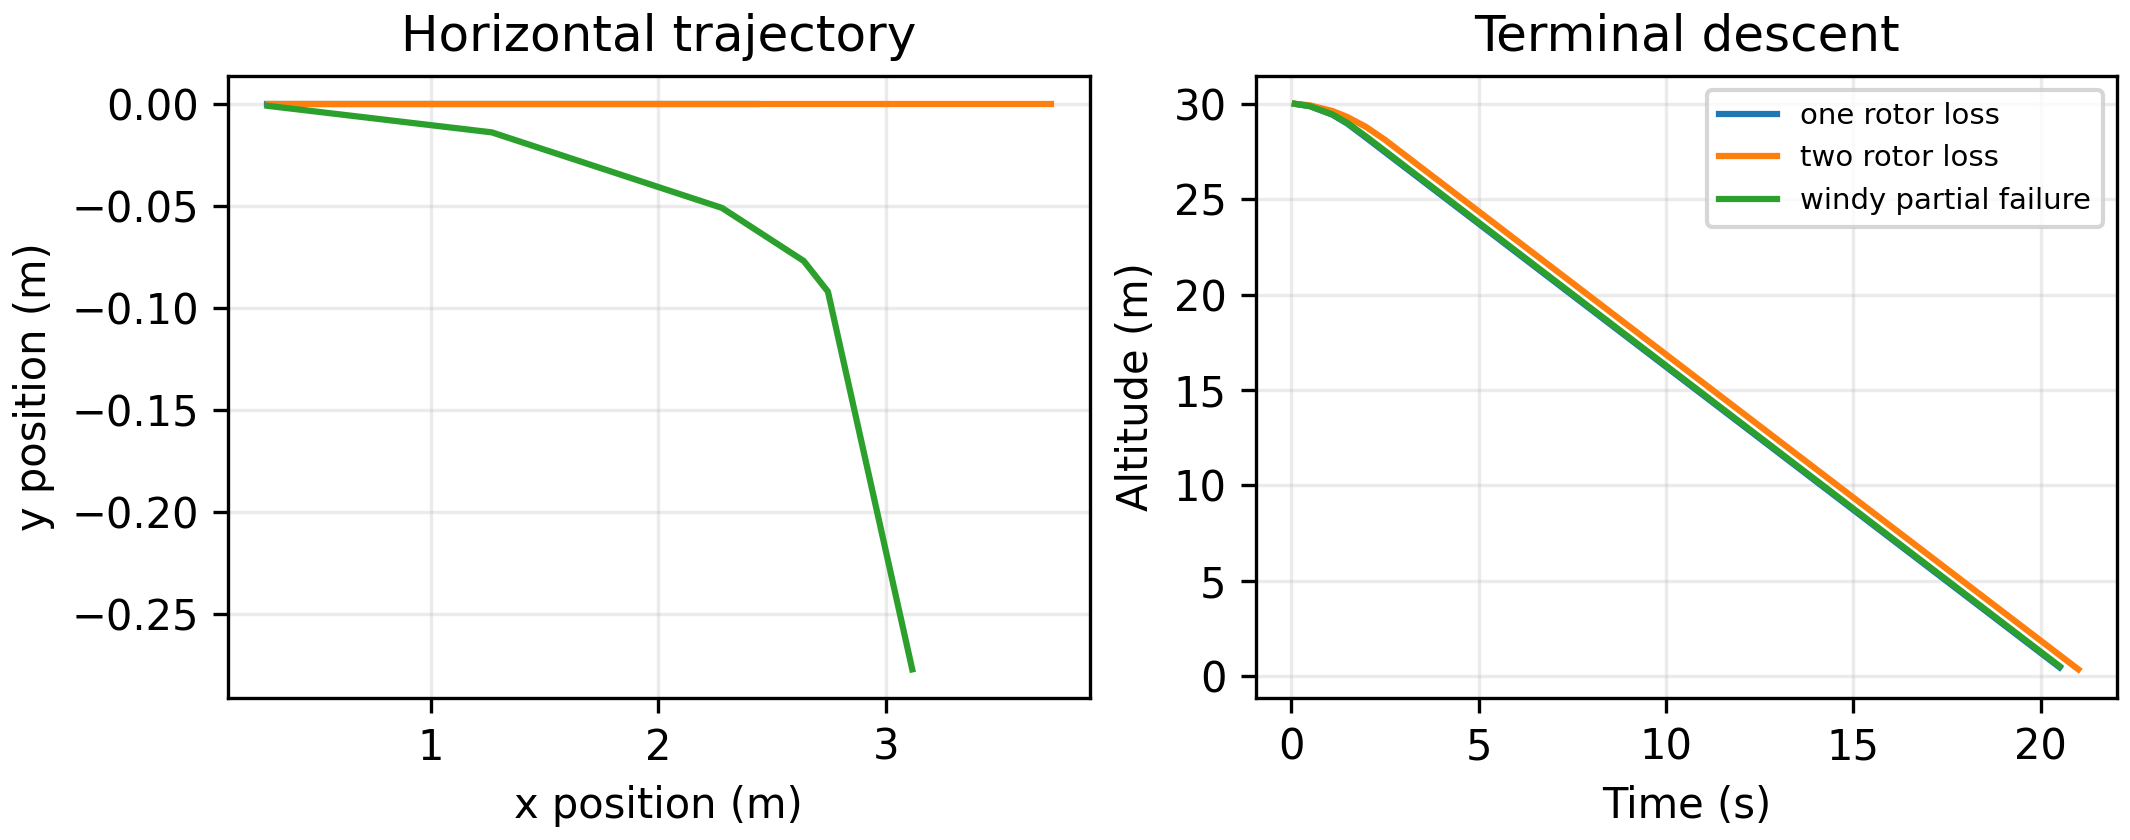
\includegraphics[width=\textwidth]{figures/trajectory_and_altitude.png}
\caption{Generated horizontal trajectories and altitude histories for the
three degraded scenarios. These are outputs of the reduced-order simulator,
not flight measurements.}
\label{fig:trajectory}
\end{figure*}

\subsection{Scenario comparison}
Table~\ref{tab:results} summarizes all three generated scenarios. The exact
JSON files are stored in the repository and can be regenerated with one
command. All three scenarios make contact within the 30-s horizon. The
two-rotor-loss scenario has lower modeled authority and therefore takes longer
to descend to contact in this baseline. The windy case demonstrates that a
small disturbance changes the terminal horizontal state even when the target
descent command is unchanged.

\begin{table}[t]
\caption{Reduced-order simulator results}
\label{tab:results}
\centering
\footnotesize
\begin{tabular}{lrrrr}
\toprule
Scenario & End time (s) & Speed (m/s) & $x$ (m) & $z$ (m)\\
\midrule
One rotor loss & 20.9 & 1.50 & 2.431 & 0.000\\
Two rotor loss & 30.0 & 1.50 & 3.721 & 1.861\\
Windy partial failure & 20.9 & 1.50 & 3.114 & 0.000\\
\bottomrule
\end{tabular}
\end{table}

The two-rotor result in Table~\ref{tab:results} is a terminal state at the
30-s horizon rather than ground contact; it should therefore not be described
as a successful landing. This distinction is important for evaluating
terminal policies and is why the JSON output includes a Boolean contact flag.

\begin{figure}[t]
\centering
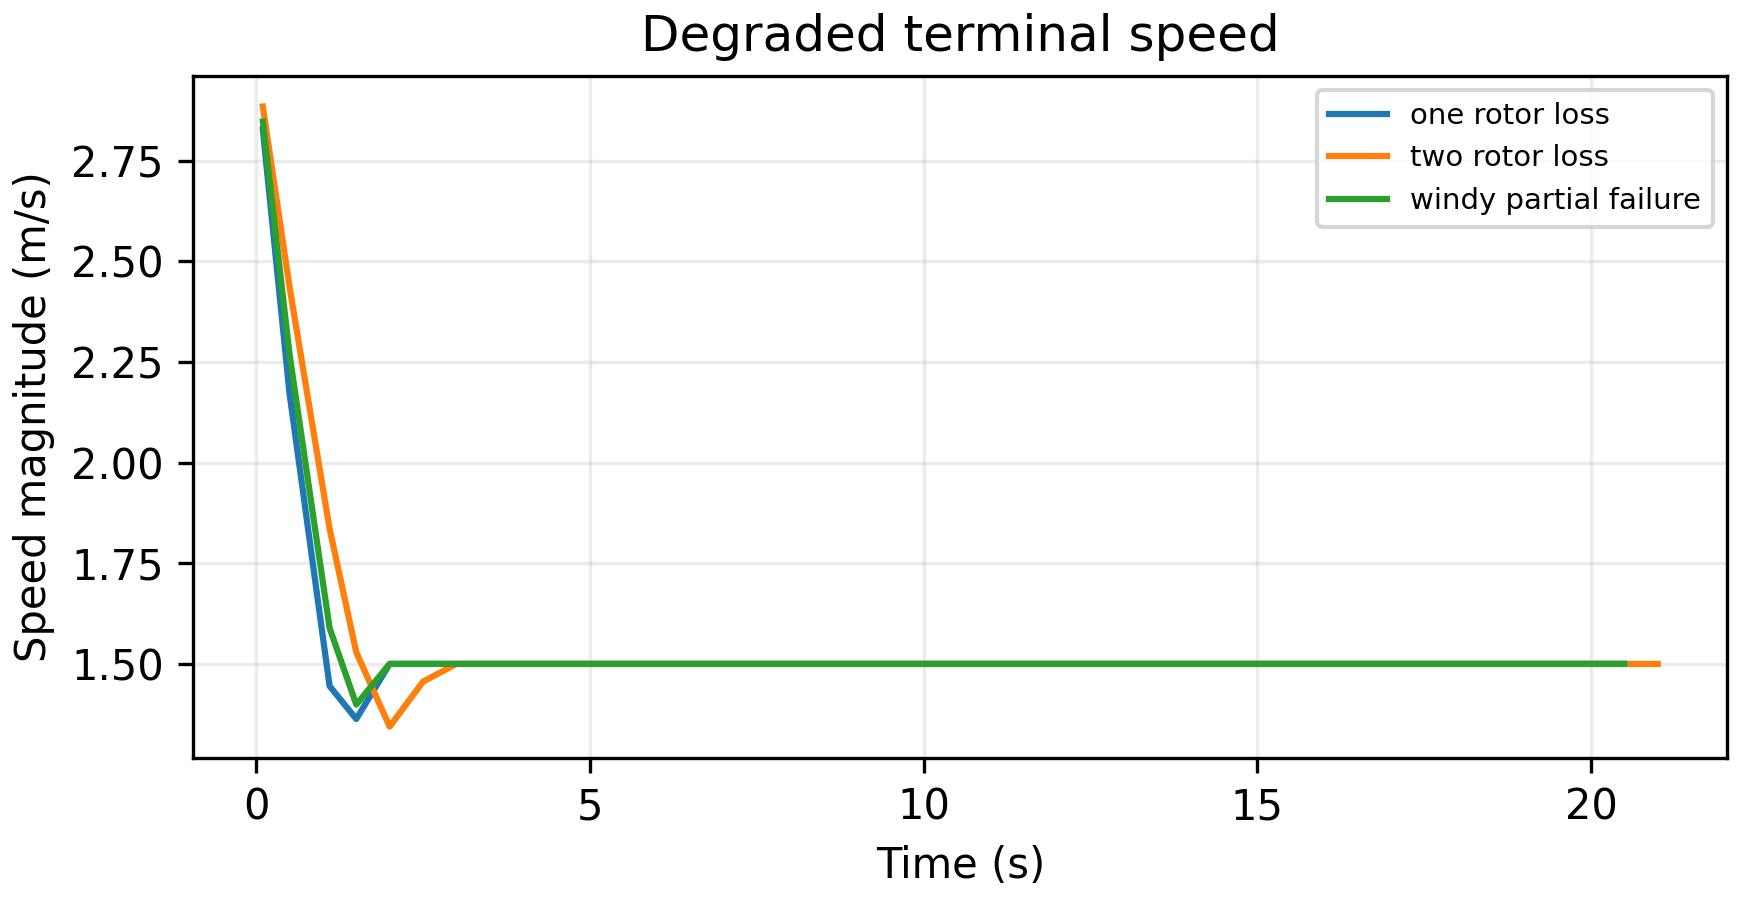
\includegraphics[width=\columnwidth]{figures/speed_comparison.png}
\caption{Speed magnitude during degraded descent. The horizontal speed is
damped while the commanded descent component becomes dominant.}
\label{fig:speed}
\end{figure}

\begin{figure}[t]
\centering
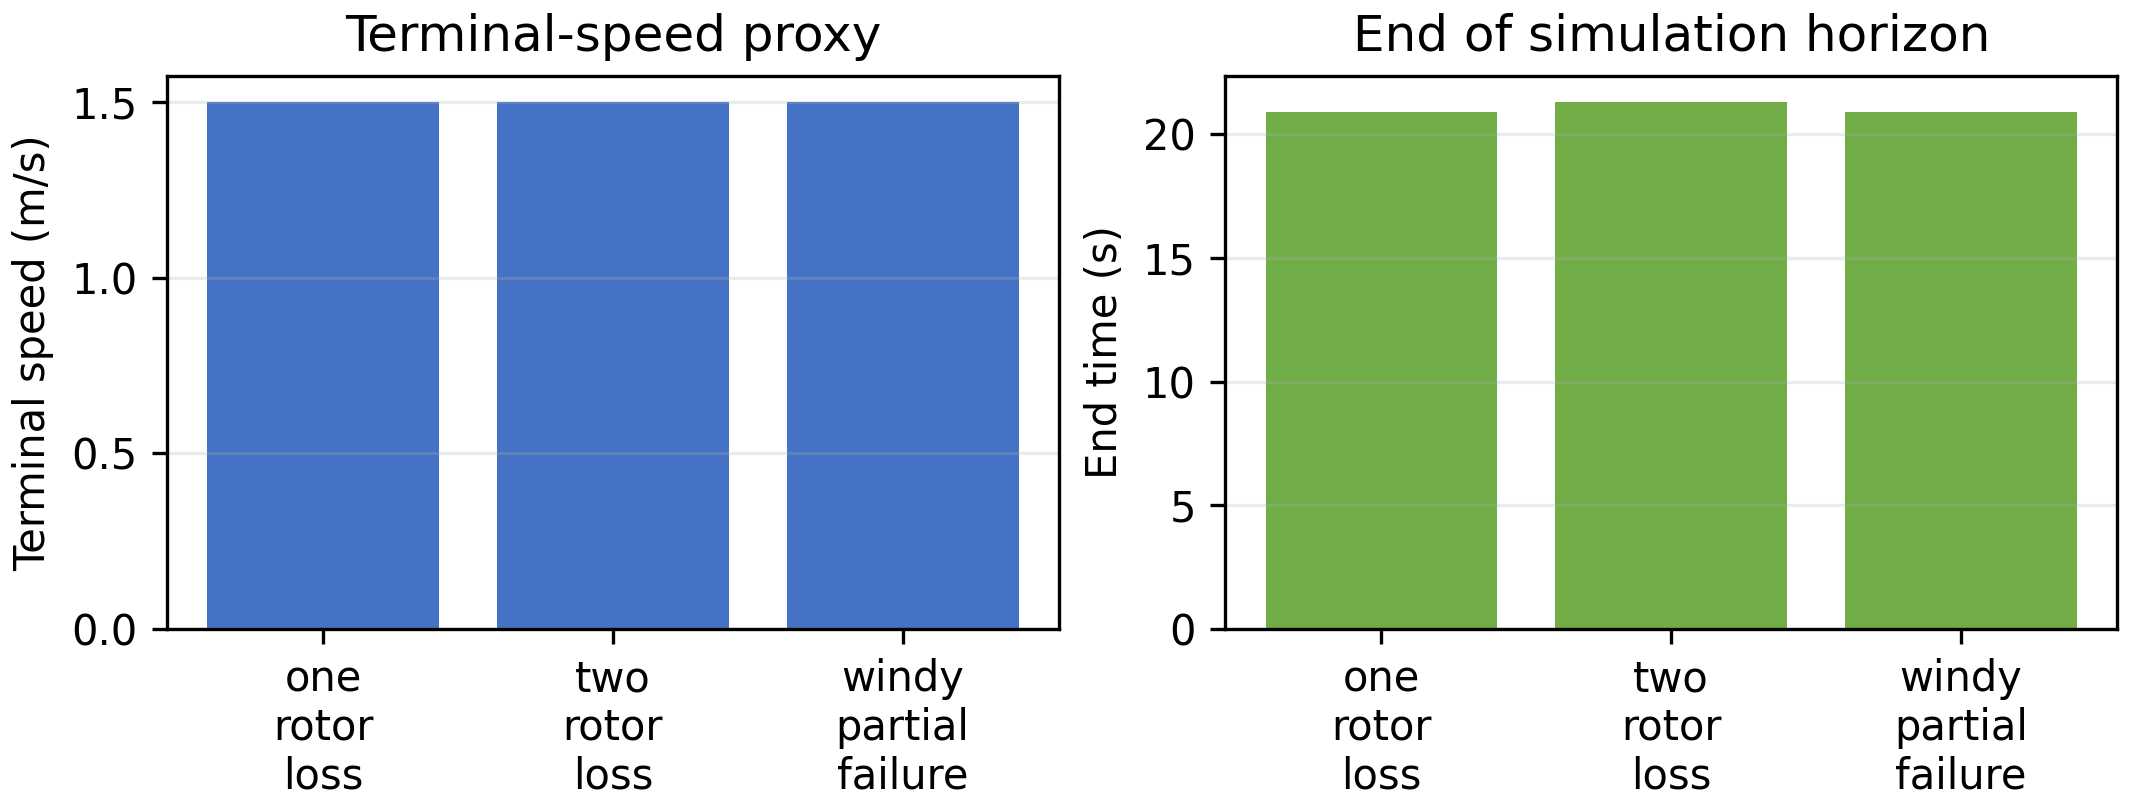
\includegraphics[width=\columnwidth]{figures/scenario_summary.png}
\caption{Scenario-level terminal-speed proxy and simulation end time. The
two-rotor-loss case does not contact the ground within the 30-s horizon.}
\label{fig:summary}
\end{figure}

\subsection{Decision-layer result}
The candidate set contains an open field, a communications corridor, and an
urban roof. The urban roof is geometrically attractive and recoverable but
violates the hard human-exposure threshold. The open field is safe but has
lower mission and communication value. The communications corridor remains
feasible and is selected by the baseline. With remaining data, adequate
communications, and a safe site, the policy selects
\texttt{transmit\_and\_observe}. This result demonstrates the intended
separation: the policy permits mission preservation only after the safety
filter has removed the high-exposure alternative.

\section{Limitations and Safety Considerations}
The model has several limitations. It is not a full six-degree-of-freedom
rigid-body simulation; it omits rotor gyroscopic effects, motor dynamics,
ground effect, aerodynamic drag identification, attitude singularities,
structural breakup, and contact mechanics. Rotor health is deterministic and
known, whereas real diagnosis is delayed and uncertain. Site attributes are
manually specified rather than generated by a calibrated perception model.
Human exposure is a scalar proxy, not a population or injury model. The
mission utility weights are illustrative and have not been elicited from an
operator or safety case.

Consequently, the results must not be used to command a real UAV. Before
hardware use, the framework requires conservative uncertainty bounds,
independent geofencing, verified emergency fallback, hardware-in-the-loop
testing, controlled impact experiments, and an aviation safety review.
Mission value must remain subordinate to protection of people and critical
infrastructure.

\section{Future Evaluation Plan}
The next evaluation should compare immediate descent, safety-only selection,
fault-tolerant tracking without mission utility, and the proposed policy over
Monte Carlo samples. Factors should include rotor-loss pattern, diagnosis
delay, wind, initial speed, altitude, site-classification error, communication
dropout, and population-density uncertainty. Primary outcomes should be
human-exposure probability, contact speed, and constraint-violation rate.
Secondary outcomes should include mission data delivered, observation quality,
payload survivability, recoverability, computation time, and regret under
model mismatch. A policy should not be considered improved if its mission
utility increases while its hard safety constraints degrade.

\section{Conclusion}
The literature establishes that a multirotor can retain meaningful
controllability after severe propeller loss and that landing-site assessment
can combine geometry, semantics, and risk. The missing system-level link is a
decision layer that treats terminal descent as a finite-horizon allocation of
remaining control authority. The framework and results presented here provide
that link in a deliberately transparent baseline. The initial experiments
demonstrate reproducible trajectory, contact, and decision outputs, while also
showing why higher-fidelity dynamics, uncertainty modeling, and validated
human-risk assessment are necessary before operational claims are possible.

\balance
\bibliographystyle{IEEEtran}
\bibliography{references}
\end{document}
